\chapter{Overview}\label{chap:overview} % (fold)
\begin{definition}{Concyrrency - 1}{}
    In computer science, \textbf{concurrency} is a property of systems in which several computational processes are executing \textbf{at the same time}, and potentially interacting with each other.
\end{definition}
\begin{definition}{Concurrency - 2}{}
    Concurrency is concerned with the fundamental aspects of systems of multiple, \textbf{simultaneously active} computing agents, that \textbf{interact} with one other.
\end{definition}
Common aspects:
\begin{itemize}
    \item systems with multiple activities or \textbf{processors} whose execution \textbf{overlaps in time};
    \item activities can have some kind of \textit{dependencies}, therefore can \textbf{interact}.
\end{itemize}
\begin{description}
    \item[Concurrent Programming] Building programs in which multiple computational activities overlap in time and typically interact in some way.
        It focuses on program organisation working on logical/abstract level.
    \item[Concurrent Program] A finite set of \textit{sequential} programs that can be executed in parallel:
        \begin{itemize}
            \item a sequential program specifies sequential execution of a list of statements;
            \item the execution of a sequential program is called \textbf{process};
            \item a concurrent program specifies two or more sequential programs that may be executed concurrently as \textit{parallel processes};
        \end{itemize}
        The execution of a concurrent program is called \textbf{concurrent computation or elaboration}.
        \item[Parallel Programming] The execution of programs overlaps in time by running on separate \textit{physical processors}
        \item[Distributed Programming] When processors are distributed over a network without shared memory, shared lock and independent failures.
\end{description}
\begin{cimage}
    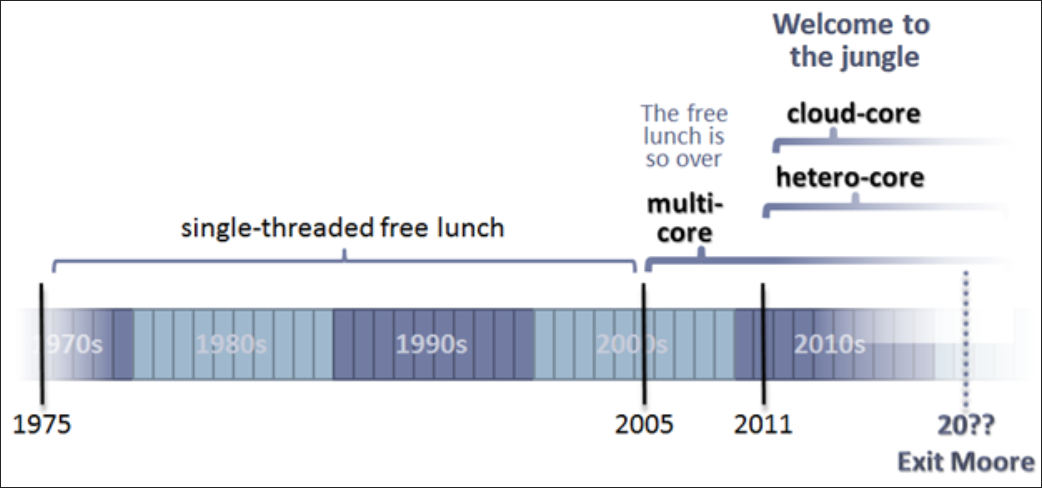
\includegraphics[width=.8\textwidth]{assets/parall-arch-timeline.png}
\end{cimage}
\section{Multi-Core Architectures}\label{sec:ow_multi_core_architectures} % (fold)
Chips having \textbf{multiprocessors} are called \textbf{multicore}: sharing RAM and possibly cache levels.
\begin{cimage}
    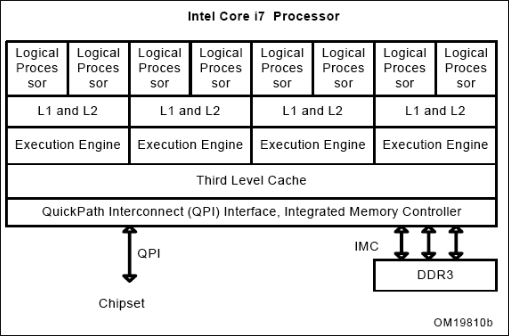
\includegraphics[width=.6\textwidth]{assets/multi-core-intel-arch.png}
\end{cimage}
%
\subsection{Hybrid Architectures}\label{sub:ow_hybrid_architectures} % (fold)
Recent architectures are \textbf{hybrid}, combining CPU cores of varying sizes:
\begin{itemize}
    \item \textbf{\ac{pcore}}: traditional design featuring high clock speeds;
    \item \textbf{\ac{ecore}}: slower but physically smaller, consume much less power;
\end{itemize}
\begin{example}{}{}
    Intel Core i9 - 14th Gen desktop processors 24 cores:
    \begin{itemize}
        \item 8 \ac{pcore} (highest performing);
        \item 16 \ac{ecore} (for background tasks);
    \end{itemize}
\end{example}
% subsection Hybrid Architectures (end)
% section Multi-Core Architectures (end)
%
\section{Parallel Computers}\label{sec:ow_parallel_computers} % (fold)
\subsection{Heterogeneous Cores}\label{sub:ow_heterogeneous_cores} % (fold)
\textbf{Heterogeneous Chips Designs} augment a standard processor with one or more specialised compute engines, called \textbf{attached processors}.
For example: \ac{gpu}, \ac{gpgpu}, \ac{fpga}, Cell Processors, \textbf{CUDA} architecture.
\begin{cimage}
    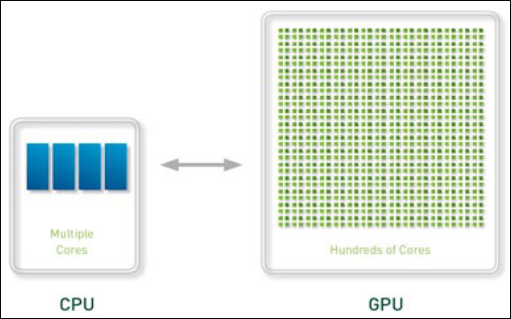
\includegraphics[width=.8\textwidth]{assets/cpu-gpu-cores.png}
\end{cimage}
% subsection Heterogeneous Cores (end)
%
\subsection{Super Computers}\label{sub:ow_super_computers} % (fold)
Traditionally used by national labs and large companies.
They use a different kind of architecture, including \textit{clusters}, having many processors (multicore) connected by ad-hoc networks.
% subsection Super Computers (end)
%
\subsection{Clusters}\label{sub:ow_clusters} % (fold)
Mad for commodity parts, nodes are boards containing one or few processors with RAM and sometimes disk storage, each one connected by commodity interconnect.
The memory is not shared among the machines: each processor communicates by message passing.
% subsection Clusters (end)
%
\subsection{Cloud Computing}\label{sub:ow_cloud_computing} % (fold)
Delivering computing \textbf{as a service} through the network: shared resources, software and information are provided to computers and other device as a metered service over a network.
% subsection Cloud Computing (end)
% section Parallel Computers (end)
%
\section{Flynn Taxonomy}\label{sec:ow_flynn_taxonomy} % (fold)
Categorization of all computing systems according to the \textit{number of instruction stream} and \textit{data stream} (\textbf{streams} are sequence of instruction or data on which a computer operate).
\begin{description}
    \item[\ac{sisd}] Von-Neumann model with a single processor computers
    \item[\ac{simd}] Single instruction stream concurrently broadcasted to multiple processors, each with its own data stream (fine grained parallelism and vector processors)
    \item[\ac{misd}] No well known systems fit this
    \item[\ac{mimd}] Each processor has its own stream of instructions operating on its own data.
        These can be then decomposed according to memory organisation:
        \begin{itemize}
            \item \textbf{shared-memory}: all processes share a single address space and communicate each other by writing and reading shared variables;
            \item \textbf{distributed memory}: each process has its own address space and communicate with other process by \textit{message passing};
        \end{itemize}
\end{description}
%
\subsection{Why Concurrent Programming?}\label{sub:ow_why_concurrent_programming} % (fold)
To \textbf{exploit parallel computers}: improving their performance (throughput and reactivity).
\emptyln{}
To \textbf{properly support} the design and development of complex \textbf{software systems}.
\begin{quote}
    It is not only a matter of mechanisms, but concepts and design methods (modularity, encapsulation, programming paradigms, etc.)
\end{quote}
% subsection Why Concurrent Programming? (end)
% section Flynn Taxonomy (end)
%
\section{A Conceptual Taxonomy}\label{sec:ow_a_conceptual_taxonomy} % (fold)
Concurrency in:
\begin{description}
    \item[System + Environment] There are two types:
        \begin{itemize}
            \item \textbf{transformational systems}: pure functional/synchronous systems;
            \item \textbf{reactive systems}: a system that computes by reacting to stimuli from its environment, with asynchronous interaction (non-termination can be a \textit{feature});
        \end{itemize}
    \item[\textit{Inside} the System] From a \textbf{structural} point of view systems as a set of ``\textbf{active components}'' + ``passive components'', the active components encapsulate a control flow.
        \emptyln{}
        From a \textbf{behavioural} point of view systems as a collection of ``\textbf{processes}'' where each process is a sequence of actions possibly non-terminating.
        \emptyln{}
        From an \textbf{interaction} point of view there are different interaction models:
        \begin{itemize}
            \item by shared memory or shared ``passive components'';
            \item by message passing;
            \item by producing and consuming events;
        \end{itemize}
\end{description}
%
\subsection{Concurrent Hyper-Cube}\label{sub:ow_concurrent_hyper_cube} % (fold)
A multidimensional space, \textbf{concurrent hyper-cube}, where to locate various approaches:
\begin{itemize}
    \item \textbf{control flow model}: synchronous or asynchronous;
    \item \textbf{shared memory} or \textbf{message passing}: message passing could be synchronous or asynchronous;
    \item \textbf{not distributed} or \textbf{distributed};
    \item \textbf{control oriented} or \textbf{data-oriented};
\end{itemize}
% subsection Concurrent Hyper-Cube (end)
% section A Conceptual Taxonomy (end)
% chapter Overview (end)
